\label{chap:implementation}
In this chapter we will discuss the main implement ion issues that arrised during the development of the project
and the approach that we took to implement the design from the previous chapter, we will begin by describing the
software tools that were used throughout the implementation, then we will discuss the implementation of the front-end
, object system and finally the back-end of the system.

\section{Tools} 
\subsection{Implementation Language}
The implementation language that we have chosen is C, specifically C11. The choice of C is because it it the
language that I am most familiar with, also it is a language that offers performance benefits as it is a compiled
language, this is of great advantage for a photon mapper as we will regularly be dealing with data structures
that contain thousands to millions of elements (such as the photon map.) In addition to being a compiled language
the memory management of the program is left to the programmer, while this can cause issues such as buffer overflows
it has the benefit of providing a great deal of control to the program writer as they can be aware of all memory
that is used by the program, which, when dealing with data structures as large as the photon map is a large benefit.

\subsection{Coding Style and Code Quality}
With any piece of software it is important to impose restrictions on the way in which the code is written in order
to reduce the effort that is needed to read the source. Some of conventions that we have used includes having a
convention for any typedef such that a type can be easily determined (appending \_t to the end of the typename),
requiring that if a function is non-static that it begin with the name of the file or another prefix to prevent
name clashing. Another convention that is used is the use of opaque pointers \cite{opaque-pointers} to data structures in order to
hide the internal data representation of the types an example of this can be found in the source files \texttt{list.h/c}
it can be seen that the header file does not expose the structure definition to any file that includes the header.

Throughout the development of the system it was necessary to use a number of tools in order to ensure the
quality of the code being produced.

Another issue that is present in writing code for C is that the memory is managed by the programmer, as a
result it is common for errors such as memory leaks to occur, in order to reduce the risk of this in the project
we have utilised several programs that can identify issues.

\subsection{Valgrind}
In order to detect memory related bugs we used Valgrind which is a program that will track all memory allocations
of a running program and is able to detect errors such as writes after a region of memory that has been allocated
and lost pointers that result in memory leaks.

\begin{figure}
\lstinputlisting[language=C]{./implementation/val.log}
\label{fig:valgrind_listing}
\caption{Example Valgrind Output}
\end{figure}

\subsection{Static Analysis}
Included with the clang compiler suite is the clang static analyser, this program will perform analysis on the
source code of a program and will report certain types of errors such as performing memory accesses on variables
that can potentially be NULL, while this may seem similar to valgrind, this approach will detect errors such
as this without running the program and can find issues that may only manifest in certain corner cases that
may not appear during testing.

\subsection{Source Control}
In order to organise the code that we have developed we decided to use Git as a source control system for the project.
Git has the concept of branches that allow development of separate features concurrently in isolation and
merged upon completion, incorporating branched into the development work flow proved to be a highly useful feature
as it allows for work on a feature to continue even if another feature breaks parts of the system that would
otherwise make continued development impossible

\subsection{Profiling}
When writing software it is desirable to optimise it in order to improve the performance of the code, this project
is no different and there are many area that could be optimised, to quote Knuth

\begin{quotation}
{Premature optimisation is the root of all evil ... in programming \cite{Knuth74a}}
\end{quotation}

This refers to the practice of optimising code that is not a bottleneck in the execution of the program, for instance
reducing the running time of a function by $50\%$ that is only executed for a small proportion of the running time of
the whole program in order to decide which parts of the code needs to be optimised we have used the combination of
the compiler profiling flag and gprof, a program that will output profiling statistics for a run of the executable,
this includes information such as the number of times a given function was called and the percentage of the run time
taken by the function.

\newpage
\section{Common Data Structures}
In this section I will briefly discuss some data structures that are used as part of the system that cannot
be catagorised as being in the front or the back end.

Due to the small standard library provided by C many features that are commonly found in more high level languages are not
found in C, for this project we need three such data structures, lists queues and vectors.

\subsection{Lists}
As we don't know how many objects and lights are in the scene and number of photons stored in the photon maps depends on the
lights and geometry in the scene, as a result we have implemented a list data structure that allows for the size of the list
to increase as elements are added to the list.

\subsection{Queue}
During the photon mapping stage of the back end we need to coordinate a number of threads that is dependant on runtime inputs,
the problems that we faced during the development were distribution of work and coolation of the results of each thread,
the solution that we decided upon in both cases was to use a thread-safe queue implementation, this is implemented as a
fixed size circular buffer, two pointers are stored to the front and back of the queue, as items are read from the queue to
front of the queue is decreased and writing to the queue increases the back pointer.

\subsection{Vectors}
Some of the most common operations that are performed during photon mapping and raytracing are vector operations.

\newpage
\section{Front End}
\section{Front End}
The front end of the system deals with the input and output of the system, this will manipulate and process
the input into a form that can be used by the back-end to perform the synthesis, separating the front and back-end
allows the i/o and the synthesis to be modified with no modification required for the other block,
for instance the output could be an BMP image or a surface within a GUI, the details of the conversion are
irrelevant to the back-end, only that the data passed to it is in a format that is understood.

\subsection{Scene Input}
The scene input takes in a description of a scene that is to be rendered from a file, this scene description
will give a listing of each of the objects in the scene such as meshes, lights and camera. Each of these
objects are also described by a file that is listed in the scene file. Each of the scene files are text files
that are human readable, this allows the files to be easily modified. Each of these configuration files allows
for attributes to be reused such as a material describing a mirrored surface can be defined in a single material
file that can be referenced by multiple objects. below is a list of the different scene files that are defined

\begin{description}
\item[.scene] Top level description of the scene
\item[.mesh] Description of a mesh, including material and surface data.
\item[.mat] Description of a objects surface properties.
\end{description}

\subsubsection{PLY mesh format}
One aspect of the mesh input file is a file-name that refers to a PLY polygonal mesh, it was decided that using
a pre-existing file format for the input to system was beneficial as it allowed for assets from 3D modelling
utilities to be used to create the test scenes as they contain the required functionality to export to PLY
meshes. the choice of the PLY made because it is a human-readable format (a binary PLY format is available but
not supported by the system) and we specify this to be a key requirement of the system, 
using PLY also allowed for example meshed from the Stanford PLY repository which in turn provided a selection of
relatively complex models that could be used during the production and testing.

\begin{figure}
\lstinputlisting[language=C]{../Code/data/scenes/cornell_box.scene}
\label{fig:scene_file_example}
\caption{Example Scene File}
\end{figure}

\subsection{Command Line Arguments}
The program that is created must be able to take in more than one scene file to be useful, by having command
line arguments this allows the scene file to be changed without recompiling the code, there are other options
that are available including the number of threads that will be used to perform the ray-tracing and the
resolution and name of the output file, this will allow for the system to be used in scripts.

\subsection{Image Output}
The image and GUI block contains the code that will take the final pixel colours and present them to the screen
there will be two modes of operation, image output and GUI output, image output saves the image to a file such
as png or bmp.

\subsection{GUI}
In order to provide immediate feedback to the user it is necessary to include a GUI in the system, this will
be a simple window that will display the progress of the system as it creates the images, this is useful
for testing changes to a scene as it may be possible to see if the change has had the desired effect without
finishing what may be a costly render or to assure the user that a render is still running, the block level
design of the GUI can be found in Figure~\ref{fig:gui_design}.

\begin{figure}
\centering
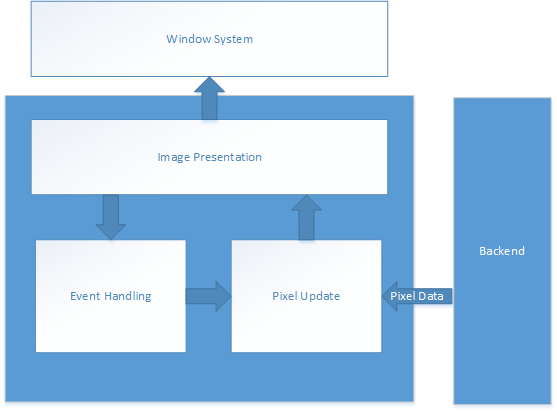
\includegraphics[width=0.7\textwidth]{./images/gui_design.png}
\caption{GUI design diagram}
\label{fig:gui_design}
\end{figure}

\subsection{Console Output and Logging}
In certain environments it is not possible to support a GUI (headless server) as a result the system includes
output on the console that inform the user of the progress of the render, this provides a visual display of the
progress at each stage in the rendering and also any warnings that can be used to debug issues that arise
during the execution of the program.

\newpage
\section{Object System}
In order to meet requirement \todo(find requirement to ref) the system needs to be able support arbitrary objects descriptions
that can be traced in the scene, this is implementatied as a structure that contains function pointers that perform functions
that must be supported by all raytracable objects and the data related to the individual object.
By encapsulating the data and the functions performed by the object it is possible to create algorithms on objects in the
abstract such that the details of the object can be ignored, for instance calculating a reflected ray at a point if intersection
is a function of only the surface normal at that point, wheither it is a triangle mesh or sphere the same ray will be calculated,
a full list of the functions that need to be defines is given in Figure~\ref{fig:object_funcs}

\begin{figure}[h]
\begin{description}
\item[int  (*intersection\_func)(object\_t *o, ray\_t *ray, intersection\_t *info)] \hfill \\
	Tests if the input ray intersectes with the object, returns the result and any other information is stored in the input variable info
\item[void (*bounds\_func)(object\_t *o, aabb\_t *bounds)] \hfill \\
	Returns the bounds of the object which is used during the scene-ray intersection test.
\item[void (*normal\_func)(object\_t *o, intersection\_t *info, double *normal)] \hfill \\
	Returns the normal of an object at a given intersection point defined in info.
\item[void (*tex\_func)(object\_t *o, intersection\_t *info, double *tex)] \hfill \\
	Returns 2-d texture coordinates in tex of the object at the point of intersection info.
\item[void (*delete\_func)(object\_t *o)] \hfill \\
	Frees any memory and other resources used by the object.
\item[void (*shade\_func)( object\_t *object, scene\_t *scene, intersection\_t *info)] \hfill \\
	Returns the colour at the surface of the object at the intersection point defined in info the result is stored in info.
\end{description}
\label{fig:object_funcs}
\caption{Functional Definition of an Object}
\end{figure}


We will now attempt to give an overview of the implementation of the objects currently used within the system.

\subsection{Sphere}
The sphere primitive is defined implicitly as an origin point and distance from the origin, including a sphere primitive is
a natural choice as many of the operations that we need to perform such as intersection tests and finding the normal at the
point of intersection is much simpler for spheres that most other surfaces allowing us to use this primitive for testing
changes while being confident that any errors that we find are not within the object definition of the sphere, the same cannot
be said for a mesh where the optimised intersection test used is fairly complex and contains more scope for implementational errors.

\subsubsection{Intersection test}
Given that we define a ray and a sphere in a parametric form it is intuitive to solve the intersection of these objects implicity,
given a ray defined $\vec{o} + t \vec{d}$ and the equation for a sphere $x ^ 2 + y ^ 2 + z ^ 2 - r ^ 2 = 0$

\subsection{Mesh}
The mesh primitive in the system is defined as a collection of vertices connected into triangles through a list of triangles,
additionally surface normals and texture coordinates can be specified in the input file (see section \todo{find section})

\subsubsection{K-D Tree Construction}
In order to satisy requirement TODO:Add the requirement bruteforce methods for raytracing are not acceptable, in order to reduce
to number of intersection tests that are performed I have decided to use the kdtree for the accelleration structure. The
construction of the kdtree is performed during the initialiseation of the triangle meshes as it is a static data structure, due
to it being a static data structure their is an advantage to performing more extensive computation in the construction in
order to create a higher quality of kdtree. TODO:Add sah and analysis. We begin the contruction of the kd-tree with all
triangles in a single list, we then calculate an axis and position on that axis to seperate the triangles, this is calculated
by \todo{add SAH or average if not implemented} we then sort each of the triangles into two child lists, if a triangle is
to the left of the splitting plane it will be placed in the left childs triagnle list and visa-versa for the right, if the
triangle spans the split plane it will be added to both lists, we then call the tree building function recursivly on the
left and right child and delete the list for this node, we terminate when a list contains less than a threshold number
of triangles in its bucket or a maximum depth is reached, or if all triangles are placed in a single node.

\subsubsection{Intersection test}


\subsection{Material Properties}
Each object has associated with it a material property that defines the reflectance properties of the material.
The system currenlty suports diffuse and pure specular components each being defined as a three floating point
values for red, green and blue compnonets respectivly, texture mapping is also supported for the diffuse component,
for specular transmission an index of refraction is defined that determins the direction of refracted rays through the
material. We also store the average values for these components explicitly as they are frequentlty used when performing
russian roulette to evaluate integrals during photon map construction and raytracing as will be seen in section \todo{Add section}

\subsubsection{Participating Media}
Materials can also be set to being a participating media, in this case we have four coefficitnes, the scattering and
absorption coefficient which will determin how light interacts with the object internally derived from these values
are the extinction coefficient and albedo we will demonstrate their useage in section \todo{section}.



\newpage
\section{Back End}
The back-end contains the code that deals with processing scene data, this block is decomposed into
two main blocks, the photon mapping block and the raytracing block, the photon mapping block is responsible
for the preprocessing step that creates the photon maps used to estimate the radiance. The raytracing stage
is responsible for computing the colour of each of the pixels in the output image, this will use the data
that was read into from the front end and the photon maps that were created by the photon map module. The
output of the raytracing block is sent to the front end which will use the data to present or save the final
image. The design of these blocks is that of a pipeline where certain procedures are performed on the scene
data and the results of the process is passed to the next stage, both pipelines contain a stage whereby
data can be passed to multiple threads to be process, each of these threads communicate to the next
stage in the pipeline through a queue that acts as the inter-thread communication method.

\subsection{Photon Emmition and Photon Map Construction (1 page)}
This block contains two stages, the photon emmition stage which traces photons through the scene and stores
the point of absorbtion and the balancing stage which sorts the photons into a data structure (left balanced
tree) that facilitated efficient storage and searching. The reason for the balancing stage is that the
distriburtion of the photons in the map is unlikely to be optimal \cite{JensenBook} and as this is a
preprocessing step it is worth the time to perform the balancing to improve later stages.

The construction of the photon map can be computationally expensive when a high number of photons are
requested to be created, in order to improve the performance of this stage multiple threads are created
that are responsible for emmitting a certain number of photons in the map, the number of threads will be
set in the front end and is configurable by the user to suit the machine that the system is being run on.

Each of the threads will trace photons through the scene as described in Algorithm\todo{Emmition Algorithm Ref}
once a photon has been found that will be stored in the photon map it will be written to a queue that is shared
by each of the threads, the photons have their power scaled as they are read from the queue.

The next stage in the pipeline reads photons from the queue, this will continue until each of the threads
has signalled that they have completed processing the photons, once all of the threads have been completed the
the list of photons will be transftered into the photon maps, this is the balancing stage.

\begin{figure}
\centering
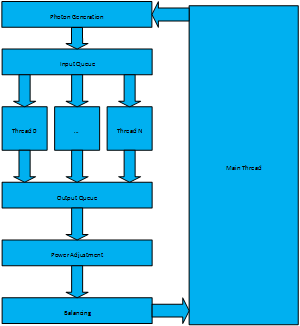
\includegraphics{./images/photon_threading.png}
\caption{Photon map generation}
\label{fig:photon_generation}
\end{figure}

\subsubsection{Multiple Photon Maps}
During the construction of the photon maps a choice must be made as to which of the photon maps the photon
should be placed in, this requires additional information to be passed from the emmition thread, this information
will describe the path that the photon has taken, this will in essence be an implementation of the path notation
that is commonly used to describe the path of a photon, in this case all paths will be stored in the global photon
map (\textbf{L(S\textbar D)$^+$D} in the path notation),only specular paths are stored in the caustic photon map
as these are the paths that contribute the most to the focusing effect of caustics (\textbf{LS$^+$D})


\subsection{Raytracing (1 pages)}
As can be seen from Figure~\ref{fig:design_blocks} the raytracing module contains $n$ threads, each of these
threads trace a subset of the pixels in the image and run independantly to each other, this is possible due
to the inherent parrellism in the photon mapping algorithm. This stage in the system will perform raytracing
as described by Shirley \cite{shirley-dist}, for each intersection found during the running of the system the photon
maps created during previous stage will be used to estimate the radiance of the point in order to estimte the
true illumination at the point factoring in the global effects.

\begin{figure}
\centering
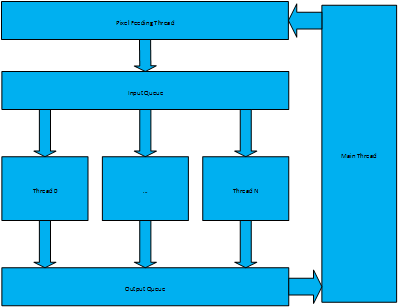
\includegraphics{./images/pixel_threading.png}
\caption{Raytracing architecture}
\label{fig:pixel_generation}
\end{figure}

The architecture of the raytracing block shared many simalarities with that of the photon emittion stage,
it is also a pipeline, there is a threads that inputs each pixel in the output image to a queue, this queue
is in turn read by one of multiple threads that perform photon mapping for a ray emmited through the pixel,
multiple rays are generated for each pixel performing distrubution raytracing, the colour of the pixel is
then written to an output queue that will be read by the main thread in order to send the pixel values to
the front end to be presented to the user.

\subsubsection{Distribution Raytracing}
Each of the raytracing threads performs distribution raytracing, this is a commonly used adjustment to the 
raytracing algorithm that allows for simulation of fuzzy phenomena such as soft shadows and glossy reflection
models, as described by Jensen \todo{cite} distribution raytracing can also be used to estimate the contribuiton
of diffuse intereflection, at each intersection of the eye ray a diffuse refeltive \todo{this is only true of
diffuse surfaces} ray is generated, this ray is then traced into the scene, at the intersection point of this ray
we use the photon map to estimate the radiance leaving the surface in the direction of the original intersection
point, as we are tracing multiple rays per pixel an estimate of the global illumination is found by averaging each
of these reflective rays.

\begin{figure}
\missingfigure{Algorithm For distributiuon raytracing}
\end{figure}

\subsection{Objects}
Much of the raytracing algorithm that is performed on each of the
objects in a scene are the same, for example finding a refracted
ray is only dependant on the surface noraml at a point of intersection
for this reason the system abstracts any object that can be intersected
must implement certain functions, this is a form of object orentation.

\subsection{Materials}
Each object has associated a material property that determines how light interacts with the surface of the
object, in this system we consider diffuse and perfectly specular materials componenets that will contribute
to the reflectance of the object, each term is split into three turns for red, green and blue components.
\todo{improve the phrasing of this}

\subsection{Participating Media}
In a simple raytracer as a ray is traced through a scene the radiance is assumed to be constant along the path,
in the real world this is not true due to lights interaction with particals in the air, these interactions
are commonly refered to as scattering, two types of scattering are possible, in and out scattering, the latter
causes a decrease in the radiance along a path and the former an increase in the scattering, this effect is
responsible for blue skies as light is scattered different amounts dependant on the frequency. In this project
the system is able to simulate this effect by applying a participating media to an object, We will only consider
the effect of scattering in three colour bands. two components are used to describe the
properties of a participating media, the scattering and absorbtion coefficient. \todo{Add some citations}

\subsection{Shading}
Each thread is responsible for performing that shading at the intersection of eye rays, for specular reflection
and transmission this results in an additional raytrace be performed to determin the shading colour, for diffuse
surfaces a direct illumination calculationn is performed, additionally the photon map is queried to determin
the indirect lighting. For participating media, the radiance is calculated by performing by a ray-marching
procedure.

\newpage
\chapter{Testing}
Testing of the program was performed in two main ways, testing of the indidual functions and testing of the system as a whole.
certain functions designed to accelerate the raytracing need to be compared to a base implementation that while slower is
guaranteed to be correct, for instance a finding the closest intersection of a ray and mesh, the simplest way to do this
is to test the ray and every triangle in the mesh and record the closest intersection, this is simple to perform and
the scope for errors in the implementation is low, unfortuanatly this is a very expensive operation that requires $\Omega(n)$
time complexity, in this project the k-d tree is used to accelerate the test, this can be performed in $\Omega(log(n))$ time
complexity, the code to perform the intersection test for this data structure is much more complicated and as a result
errors in the implementation are more likely. Testing of these complicated functions was done by comparing the output
of the simple function with the faster implementation this can be used to ensure that the outputs match, it can also be
used to see if the new implementation does indeed increase the performance of the code. Figure~\ref{fig:testing_performance_comp}

\section{System Testing}
\begin{figure}[h!]
\missingfigure{Performance Comparison}
\label{fig:testing_performance_comp}
\caption{Performance difference for triangle intersections}
\end{figure}

\subsection{Photon Viewer}
As the development of the system was performed roughly in the order described in the document, the photon map was produced before the
system used it in the radiance estimate when creating the images, as a result the result the verifiing the results of the photon
map generator posed a paticular challange as it typically contained thousands of photons in a geometry independant data structure, as
part of the development of the product we created a companion utility to the main system that allows for the visualisation of the
photon map, when inputed into the program we can see if the results match the expectation of the distribition of the photons for a
given scene. The photon viewer is reads in data from a simple format containing as a first line the number of photons and then
a list of the same length of photon positions, powers and incident directions. This tool proved to be of great value also being used
to test the sampling functions. The design of the photon viewer is simalar to that of the main GUI, differring in that it displays points
stored in an OpenGL display list \cite{khronos:2014:online}  (used to lower the number of draw calls) as oppose to rendering a
texture of the output image as in the main GUI.

\begin{figure}
\centering
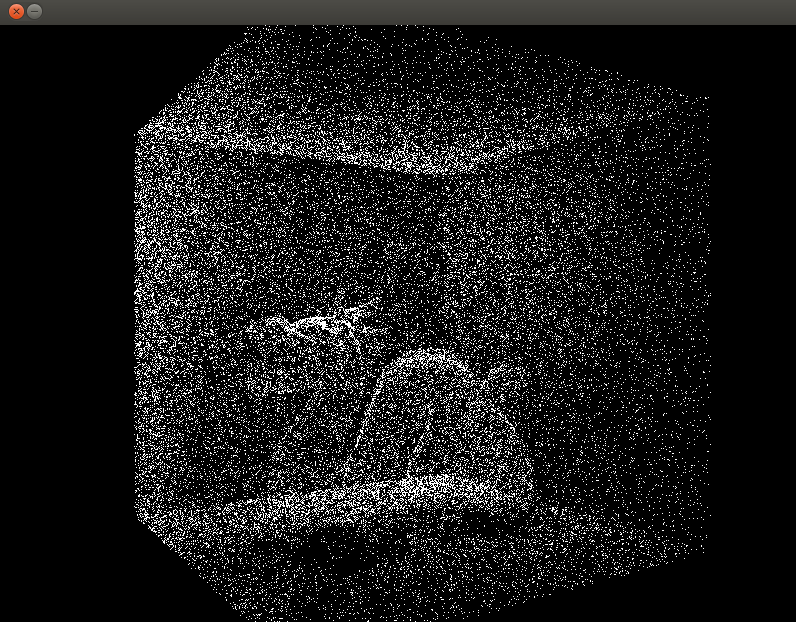
\includegraphics[width=0.7\textwidth]{./images/photon_viewer.png}
\label{fig:photon_viewer}
\caption{Photon Viewer Running}
\end{figure}

\subsection{Pixel Tracing}
When performing tests on the system it would frequenetly be the case that a change introduced obvious error in the output image,
it became apparant early in the development that being able to trace a single pixels path through the scene would make the
task of debugging that much easier. This functionallity is available as the \texttt{--trace\_pixel} option.

\section{Peformance Testing}
During the design and implementation of the system we have stated that certain descitions were made in order to improve the performance
of the system, in this section we will present results of testing that was performed in order to evaluate the gains from these descitions.

\subsection{Photon Nearest Neighbour Search}

\subsection{K-D tree intersection acceleration}

\subsection{Multicore Scaling}
In Chapter \todo{Reqs} and \todo{Design} we highlighted the inherent parralism possible in the
photon mapping algorithm in both the photon generation and raytracing stages, in order to
test the performance of the system and its ability to scale with more resources we decided to
aquire access to Amazon EC2 compute clusters, allowing us to run the system on up to 32 Intel
Xeon E5-2670 cores and 60GB of RAM \cite{amazon-instances}, we tested the system with various
settings such as resolution and number of photons in the photon map and in the radinace estimate
, each configuration will be run multiple times in order to reduce variance due to the hardware.


